\subsection{Governance}\label{sec:governance}

Polkadot uses a sophisticated governance mechanism that allows it to evolve gracefully over time at the ultimate behest of its assembled stakeholders. A key and unfailing rule is that \emph{all changes to the protocol must be agreed upon by stake-weighted referendum -- the majority of stake always commands the network.}

In order to make any changes to the network, the idea is to compose stakeholders (i.e. all holders of dots) and the Council (\autoref{s:council}) together to administrate a network upgrade decision. No matter whether the proposal is submitted by a stakeholder or the Council, it will ultimately have to go through a referendum to let all stakeholders, weighted by stake, make the decision.

Each stakeholder in Polkadot has the right to: a) submit a proposal, b) endorse a public proposal to prioritize it in the referendum timetable, c) vote on all active referenda, d) become a candidate for the Council, and e) vote on candidates for the Council. In addition, any stakeholder has the right to become a nominator or a validator candidate, to participate in NPoS (\autoref{sec:validators}).

\subsubsection{Proposals and Referenda}

The core of the Polkadot logic is stored on-chain in an amorphous state-transition function and defined in a platform-neutral language: WebAssembly. Each proposal takes the form of a privileged function call in the runtime, that is able to modify the runtime code itself, achieving what would otherwise require a "hard fork". A proposal is then tabled and associated to a referendum. 

Proposals can be started in one of several ways:
\begin{itemize}
\item a public proposal, which is submitted by any stakeholder;
\item a Council proposal, submitted by the Council with either majority or unanimous approval;
\item a proposal submitted automatically as part of the enactment of a prior referendum, and
\item an emergency proposal submitted by the Technical Committee (\autoref{s:council}) and approved by the Council.
\end{itemize} 

Each proposal approved by referendum has an associated enactment delay, i.e. a time interval between the referendum ending and the changes being enacted. For the first two types of proposals above this is a fixed interval, tentatively set to 28 days. For the third type, it can be set as desired. Emergency proposals deal with major problems with the network which need to be fast-tracked, and hence will have a shorter enactment delay. After the enactment delay, the call to the associated privileged function is automatically made.

Any stakeholder can submit a \emph{public proposal} by depositing a fixed minimum amount of dots, which stays locked for a certain period. If someone agrees with the proposal, they may deposit the same amount of tokens to endorse it. Public proposals are stored in a priority queue, and at regular intervals the proposal with the most endorsements gets tabled for a referendum. The locked tokens are released once the proposal is tabled.

\emph{Council proposals} are submitted by the Council, either by majority approval or by unanimity, and are stored in a separate priority queue where the priority is set at the Council's discretion. 

\alfonso{}{We should explain what happens to the automatic proposals -- do they go to the public-propsal queue or the Council-proposal queue, or a different queue? I don't know, we need to ask Gavin.}

A referendum is a simple, inclusive, staked-weighted voting scheme. It has a fixed voting period, after which votes are tallied. Referenda are always binary: voting options are "aye", "nay", or abstaining entirely.

\paragraph{Timetables:} Every thirty days, a new proposal will be tabled and a referendum will come up for a vote. The proposal to be tabled is the top proposal from either the public-proposal queue or the Council-proposal queue, alternating between the two queues if both are non-empty. If both queues are empty, the slot is skipped in the referendum timetable. Multiple referenda cannot be voted upon in the same time period, except for emergency referenda, which follow a parallel timetable.

\paragraph{Vote counting:} Voting on referenda is open to all stakeholders, with a voting power proportional to the stake, up to a possible vote multiplier which we explain now. A voter generally must lock their tokens up for at least the enactment delay period beyond the end of the referendum. This is in order to ensure that some minimal economic buy-in to the result is needed and to dissuade vote selling. It is possible to vote without locking at all, but in that case the voting power is a small fraction of a normal vote for the given stake. Conversely, Polkadot will offer \emph{voluntary extended locking}, that allows a voter to increase their voting power by extending the period of time they are willing to lock up their tokens. This ensures that voters committed to the system long term, who are willing to increase their exposure to the decision of a referendum, have a greater say in the matter. In particular parachains, who lock tokens when they join the network (\autoref{s:pAllocation}), as well as validators and nominators, who lock their stake to participate in NPoS (\autoref{sec:validators}), may vote with their locked tokens and automatically benefit from a vote multiplier.

\paragraph{Turnout biasing:} It may seem restrictive to force a stakeholder-based process to do something as little as, say, nudging the block time down by $5\%$. However, without this rule the network would likely be unstable, as placing its control outside of the hands of stakeholders would create a misalignment that may lead to inaction or worse. However, by taking advantage of the fact that turnout is rarely $100\%$, we can effect different outcomes depending on the circumstances, crafting a balance of power between active and passive stakeholders. For example, simple voting systems typically introduce a notion of quorum, whereby a minimum amount of turnout must be reached before a change is passed. For public proposals, we generalize this notion into a "positive turnout bias", where additional turnout always makes change more likely, assuming the same yay-to-nay ratio. Additionally, we favor the nay side (or status quo) by requiring a super-majority approval. This works on two principles: Firstly that the status quo tends to be safer than any change, and thus should have some bias towards it. Secondly that, like all means of empirical measurement, there is inevitably going to be some degree of inaccuracy and volatility over time -- a result could be $51\%-49\%$ one month and then change to $49\%-51\%$, and given the costs involved in enacting the changes of a proposal, it is advantageous to ensure that a result would not likely flip shortly after enactment. 

\begin{figure}[h!]
  \centering
  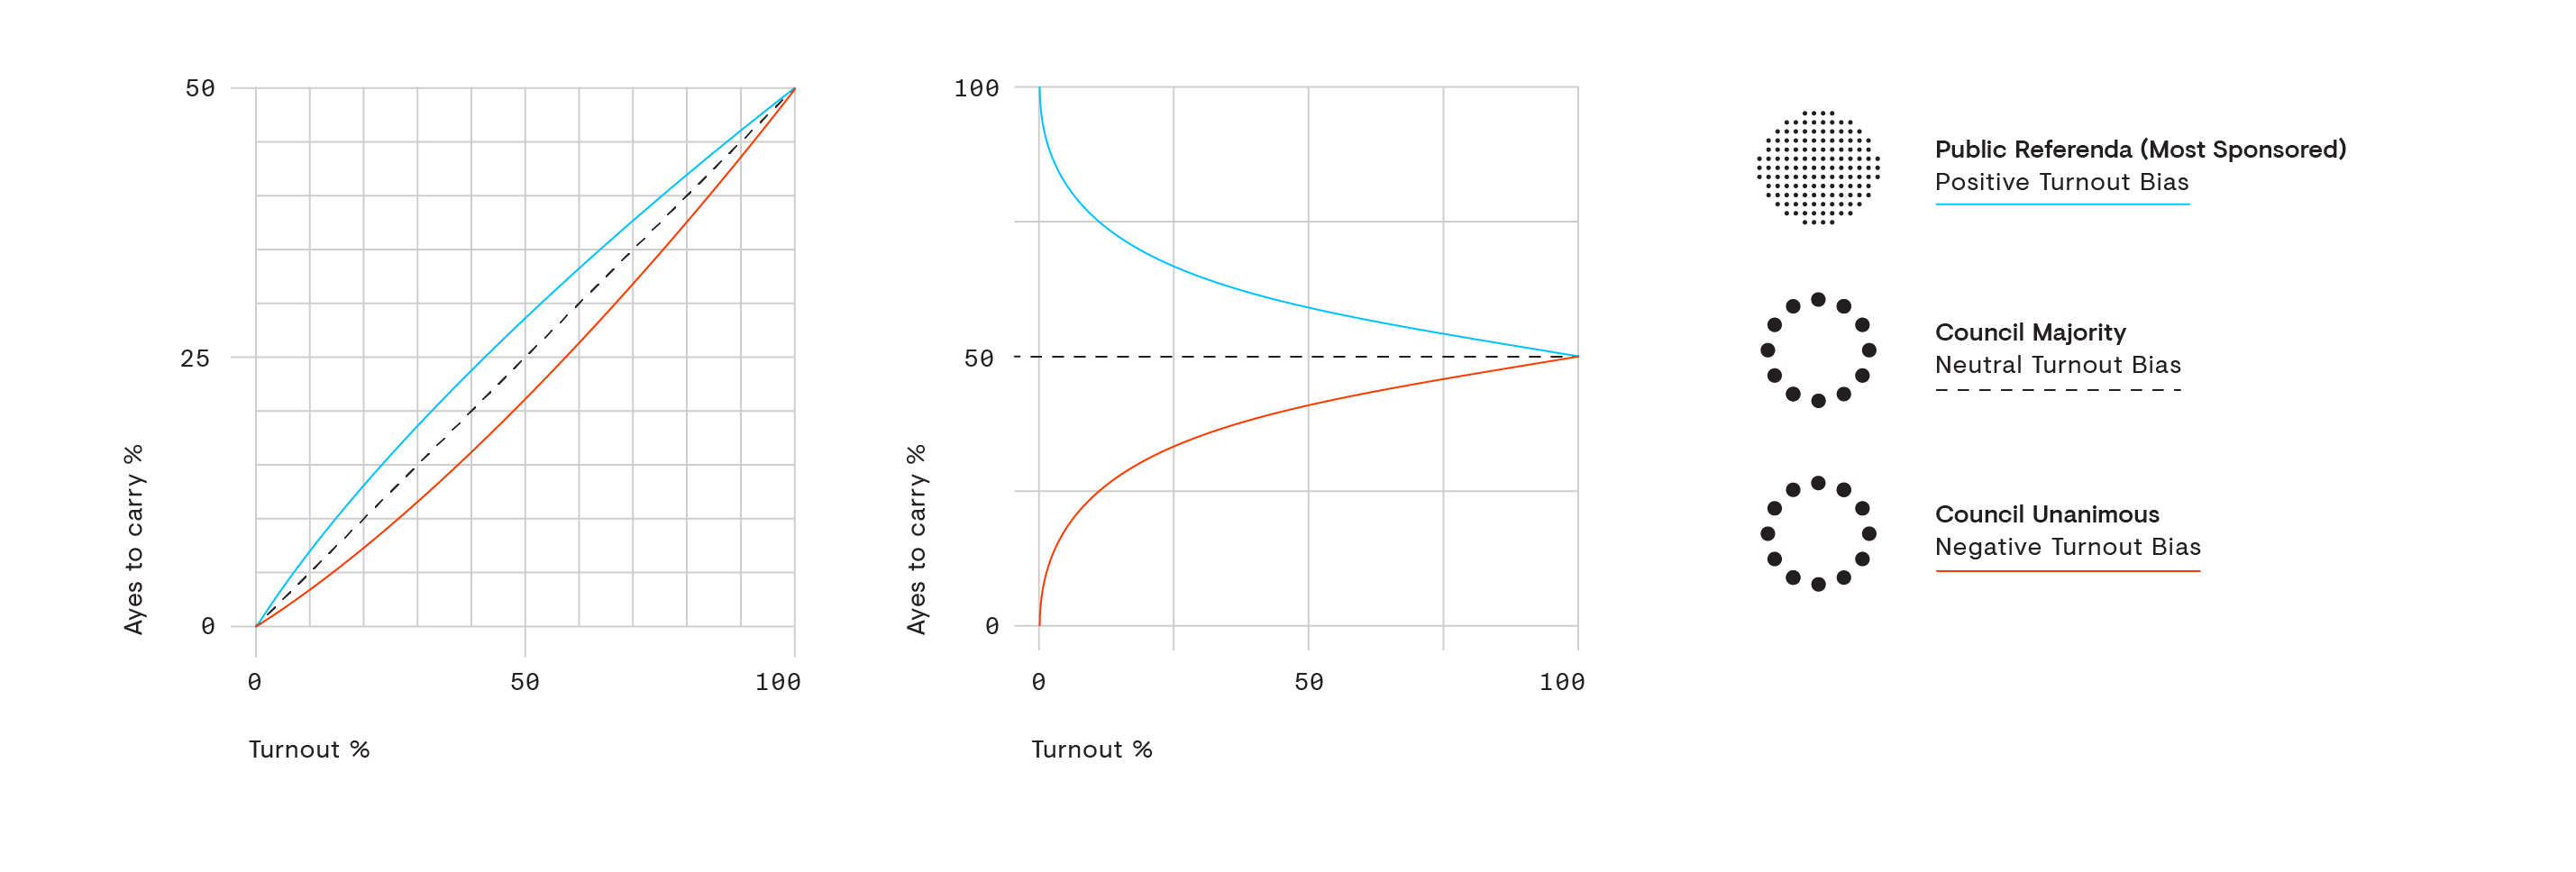
\includegraphics[width=1.1\textwidth]{images/Turnout-Bias.png}
  \caption{Adaptive turnout biasing \alfonso{}{to be replaced by a more technical figure}}
    \label{fig:biasing}
\end{figure}

\subsubsection{The Council and Technical Committee}\label{s:council}

The Council is an entity comprising a number of actors each represented by an on-chain account. Its goals are to represent passive stakeholders, organize the timetables of referenda, and review the viability and priority of proposals.

Polkadot will likely begin with six seats in the Council, and add an extra individual every two weeks, ultimately settling at 24 seats. Each member has a fixed terms, tentatively of 12 months. 

\alfonso{Each of the members is elected through approval voting.}{Not sure if I should mention which method, currently Phragmen, as I'm not sure if we will settle on that.} All stakeholders are free to launch their candidacy for a seat in the Council as well as signal their approval of any of the registered candidates. Members can be removed early only by a referendum.

\subsubsection{Allocation of parachain slots}\label{s:pAllocation}

We use auctions to have a fair and transparent parachain allocation procedure.
Since implementing seal-bid auctions are difficult and \eray{to}{we want to} avoid bid sniping\eray{}{,} we adopt \eray{an}{a} Candle auction \cite{Fuellbrunn:2012:CandleAuction} with a retroactively determined close as follows.

Once the auction has started within a fixed window\eray{}{,} bidders can post bids for the auction.
Bids go into the block as transactions.
Bidders are allowed to submit multiple bids.
Bids that a bidder is submitting either should intersect with all winning bids by same bidder or be contiguous with winning bids by the same bidder.
If an incoming bid is not changing the winners\eray{}{,} it is ignored.

For 4 lease periods\eray{}{,} we have 10 possible ranges.
We store the winner for each one of the 10 ranges in a designated data structure.
We need to make sure that a new bid does not have a gap with a winning bid on another interval from the same bidder.
This means that once a bidder has won a bid for a given range, say for example, lease periods 1-2\eray{}{,} \eray{}{-comment: What does the 1-2 notation refer to? 1 and 2?-} then he cannot bid on lease period 4 unless someone overbids him for lease periods 1-2.

For any incoming bid\eray{}{,} the new winner is calculated by choosing the combination of bids\eray{}{,} where the average deposit for overall all 4 lease periods is \eray{most}{the highest}.
Once a bid is added to the block, the amount of their bid gets reserved.

Once a fixed number of blocks have been produced for the auction\eray{}{,} a random \eray{numbers}{number} decides which one of the previous blocks was the closing block\eray{}{,} and we return the winners and their corresponding ranges for that closing block.
The reserved funds of losers are going to be released once the ending time of the auction is determined\eray{}{,} and the final winners are decided.

For example, let us assume we have three bidders that want to submit bids for a parachain slot.
\eray{Bidder $B_1$ submits the bid (1-4,75 \eray{DOT}{DOTs}), bidder $B_2$ submits (3-4, 90 DOTs), and bidder $B_3$ submits (1-2, 30 \eray{}{DOTs}).}{-comment: I do not understand the notation (3-4, 90 DOTs). -}
In this example bidder $B_1$ wins because if bidder $B_2$ and bidder $B_3$ win each unit would only be locked for an average of 60 DOTs or something else equivalent to 240 \eray{DOT-intervals}{-comment:What is a DOT-interval?-}, while of bidder $B_1$ wins each unit is locked for 75 DOTs.

 \paragraph{Treasury\eray{}{:}}

 The system needs to continually raise funds, which we call the treasury.
 These funds are used to pay for developers that provide software updates, apply any changes decided by referenda, adjust parameters, and generally keep the system running smoothly.

Funds for treasury are raised in two ways:

\eray{
1.  by minting new tokens, leading to inflation, and
2.  by channelling the tokens set for burning from transaction fees and slashing.
}
{
\begin{enumerate}
\item By minting new tokens, leading to inflation.
\item By channelling the tokens set for burning from transaction fees and slashing.
\end{enumerate}
}

 
Notice that these methods to raise funds mimic the traditional ways that \eray{governements}{governments} raise funds: by minting coins which leads to controlled inflation, and by collecting taxes and fines.

We could raise funds solely from minting new tokens, but we argue that it makes sense to redirect \eray{into treasure the tokens}{the tokens into the treasury} from transaction fees and slashing that would otherwise be burned\eray{:}{.}
\eray{ - }{-remove-}By doing so\eray{}{,} we reduce the amount of actual stake burning, and this gives us better control over the inflation rate (notice that stake burning leads to deflation, and we \eray{can’t}{cannot} control or predict the events that lead to burning).

\eray{ - }{-remove-}Following an event that produced heavy stake slashing, we might often have to reimburse the slashed stake, if there is evidence of no wrongdoing. Thus\eray{}{,} it makes sense to have the dots \eray{availabe in}{available in the} treasury, instead of burning and then minting.

\eray{ - }{-remove-}Suppose that there is a period \eray{in which there is}{with} an unusually high amount of stake burning, due to either misconducts or transaction fees. This fact is a symptom that there is something wrong with the system, \eray{that}{which} needs \eray{fixing}{to be fixed}. Hence, this will be precisely a period when we need to have more funds available in \eray{}{the} treasury to afford \eray{the}{-remove-} \eray{}{potential} development costs to fix the problem.

\eray{}{-comment:remove extra space between subsections.-}